\documentclass[a4paper,showframe,11pt]{report}\usepackage[]{graphicx}\usepackage[]{color}
%% maxwidth is the original width if it is less than linewidth
%% otherwise use linewidth (to make sure the graphics do not exceed the margin)
\makeatletter
\def\maxwidth{ %
  \ifdim\Gin@nat@width>\linewidth
    \linewidth
  \else
    \Gin@nat@width
  \fi
}
\makeatother

\definecolor{fgcolor}{rgb}{0.196, 0.196, 0.196}
\newcommand{\hlnum}[1]{\textcolor[rgb]{0.063,0.58,0.627}{#1}}%
\newcommand{\hlstr}[1]{\textcolor[rgb]{0.063,0.58,0.627}{#1}}%
\newcommand{\hlcom}[1]{\textcolor[rgb]{0.588,0.588,0.588}{#1}}%
\newcommand{\hlopt}[1]{\textcolor[rgb]{0.196,0.196,0.196}{#1}}%
\newcommand{\hlstd}[1]{\textcolor[rgb]{0.196,0.196,0.196}{#1}}%
\newcommand{\hlkwa}[1]{\textcolor[rgb]{0.231,0.416,0.784}{#1}}%
\newcommand{\hlkwb}[1]{\textcolor[rgb]{0.627,0,0.314}{#1}}%
\newcommand{\hlkwc}[1]{\textcolor[rgb]{0,0.631,0.314}{#1}}%
\newcommand{\hlkwd}[1]{\textcolor[rgb]{0.78,0.227,0.412}{#1}}%
\let\hlipl\hlkwb

\usepackage{framed}
\makeatletter
\newenvironment{kframe}{%
 \def\at@end@of@kframe{}%
 \ifinner\ifhmode%
  \def\at@end@of@kframe{\end{minipage}}%
  \begin{minipage}{\columnwidth}%
 \fi\fi%
 \def\FrameCommand##1{\hskip\@totalleftmargin \hskip-\fboxsep
 \colorbox{shadecolor}{##1}\hskip-\fboxsep
     % There is no \\@totalrightmargin, so:
     \hskip-\linewidth \hskip-\@totalleftmargin \hskip\columnwidth}%
 \MakeFramed {\advance\hsize-\width
   \@totalleftmargin\z@ \linewidth\hsize
   \@setminipage}}%
 {\par\unskip\endMakeFramed%
 \at@end@of@kframe}
\makeatother

\definecolor{shadecolor}{rgb}{.97, .97, .97}
\definecolor{messagecolor}{rgb}{0, 0, 0}
\definecolor{warningcolor}{rgb}{1, 0, 1}
\definecolor{errorcolor}{rgb}{1, 0, 0}
\newenvironment{knitrout}{}{} % an empty environment to be redefined in TeX

\usepackage{alltt}
\usepackage{standalone}
\standalonetrue
\ifstandalone
  \usepackage{../../haziq_thesis}
  \usepackage{../../haziq_maths}
  \usepackage{../../haziq_glossary}
  \addbibresource{../../bib/haziq.bib}
  \externaldocument{../01/.texpadtmp/introduction}
\fi




\IfFileExists{upquote.sty}{\usepackage{upquote}}{}
\begin{document}

In this section, a comparison between a standard random effects model and the I-prior approach for estimating varying intercept and varying slopes model is illustrated. We consider a data set which accompanies the MLwiN software on the academic achievements of 4,059 pupils at 65 inner-London schools citep{rasbash2012user, R2MLwiN}. The response variable of interest are the pupils' (normalised) GCSE scores at age 16 encoded in the variable \code{normexam}. Also available in the data set is a pupil-specific regressor, which is the London reading test results (\code{standlrt}) for each pupil taken when they were aged 11.

\begin{knitrout}
\definecolor{shadecolor}{rgb}{1, 1, 1}\color{fgcolor}\begin{kframe}
\begin{alltt}
\hlstd{R> }\hlkwd{data}\hlstd{(tutorial,} \hlkwc{package} \hlstd{=} \hlstr{"R2MLwiN"}\hlstd{)}
\hlstd{R> }\hlkwd{str}\hlstd{(tutorial[,} \hlkwd{c}\hlstd{(}\hlstr{"normexam"}\hlstd{,} \hlstr{"school"}\hlstd{,} \hlstr{"standlrt"}\hlstd{)])}
\end{alltt}
\begin{verbatim}
## 'data.frame':	4059 obs. of  3 variables:
##  $ normexam: num  0.261 0.134 -1.724 0.968 0.544 ...
##  $ school  : Factor w/ 65 levels "1","2","3","4",..: 1 1 1 1 1 1 1 1..
##  $ standlrt: num  0.619 0.206 -1.365 0.206 0.371 ...
\end{verbatim}
\end{kframe}
\end{knitrout}


First, we consider the varying intercept model. A standard approach to fitting this model is the random intercept model, which is based on the assumption that the intercepts are iid normal with zero mean. In \proglang{R}, packages such as \pkg{lme4} are able to fit these types of models. In the I-prior approach, the response variable \code{normexam} is regressed against the covariate \code{school} indicating the school that pupil had attended, which is assumed to have a nominal effect on GCSE scores. In other words, the regression function lies in the Pearson RKHS. As the variable \code{school} is a factor-type variable, the \pkg{iprior} package knows to treat this variable with the Pearson kernel automatically without user specification.

\begin{knitrout}
\definecolor{shadecolor}{rgb}{1, 1, 1}\color{fgcolor}\begin{kframe}
\begin{alltt}
\hlstd{R> }\hlcom{# Model 1: Varying intercept model}
\hlstd{R> }\hlstd{(mod1.fit} \hlkwb{<-} \hlkwd{iprior}\hlstd{(normexam} \hlopt{~} \hlstd{school,} \hlkwc{data} \hlstd{= tutorial))}
\end{alltt}
\end{kframe}
\end{knitrout}
\vspace{-0.5em}{\setlength\parindent{0pt}(output omitted)}
\begin{knitrout}
\definecolor{shadecolor}{rgb}{1, 1, 1}\color{fgcolor}\begin{kframe}
\begin{verbatim}
## 
## Call:
## iprior(formula = normexam ~ school, data = tutorial)
## 
## RKHS used: Pearson, with a single scale parameter.
## 
## Parameter estimates:
##   (Intercept)        lambda           psi 
## -0.0001139137  0.0006998747  1.1799071249
\end{verbatim}
\end{kframe}
\end{knitrout}

In Figure \ref{fig:plot}(a), the posterior means of the intercepts are plotted for the random effects model and the I-prior model. It can be seen that the estimates are in broad agreement, with conspicuously different estimates for schools 48 (-0.13 vs. -0.38) and 54 (-0.40 vs. -0.58), the I-prior giving the larger estimate in absolute values in both cases. The reason for this is that the I-prior variance for each school's regression function in a Pearson RKHS is inversely proportional to the sample size for that school. A proof of this is given in Appendix \ref{apx:pears}. Indeed, schools 48 and 54 have the smallest sample sizes of all schools, namely 2 and 8 respectively, whilst the next smallest is school 37 with 22 students.

\begin{knitrout}
\definecolor{shadecolor}{rgb}{1, 1, 1}\color{fgcolor}\begin{figure}

{\centering 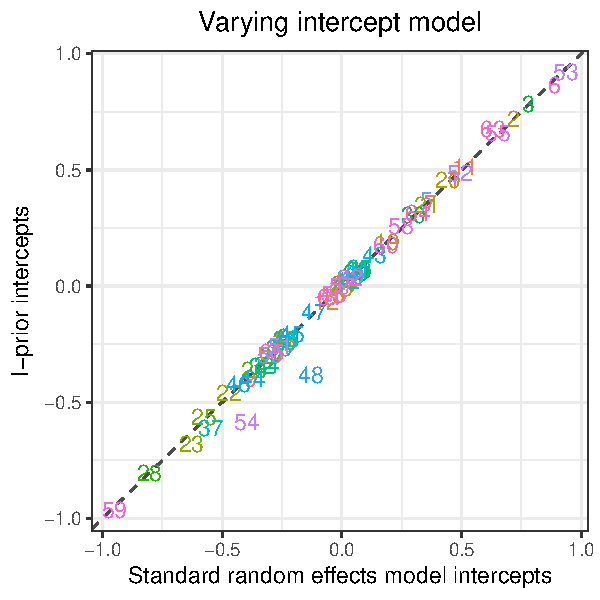
\includegraphics[width=7.1cm,height=7.1cm]{figure/04_01_plot_em-1} 
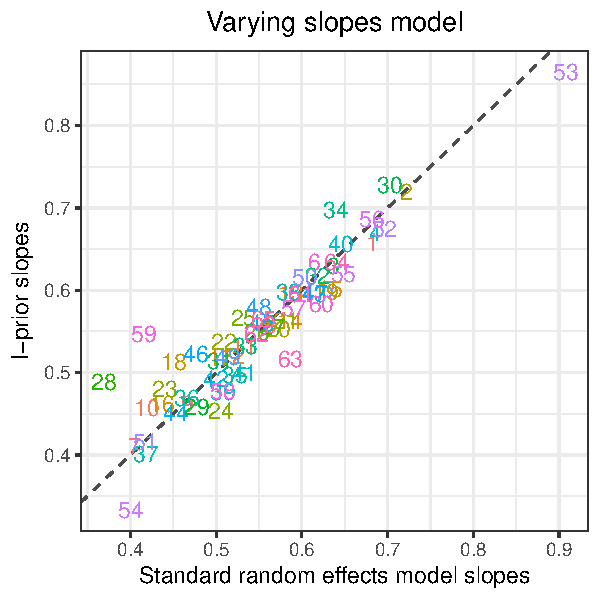
\includegraphics[width=7.1cm,height=7.1cm]{figure/04_01_plot_em-2} 

}

\caption[Estimated intercepts and slopes for school achievement data under (a) varying intercept (left)]{Estimated intercepts and slopes for school achievement data under (a) varying intercept (left); and (b) varying slope model. The numbers plotted are the school indices with the identity line for reference.}\label{fig:04_01_plot_em}
\end{figure}


\end{knitrout}

Next we consider the varying slope model which regresses, for each school, the GCSE score on the results of the London reading test taken at age 11 (\code{standlrt}). A standard approach to fitting this model is the random intercept/slopes model, which is based on the assumption that the intercept/slope pairs are iid bivariate normal with zero means. To obtain an I-prior, we assume as above a nominal effect of school, and a linear effect of \code{standlrt} (using the canonical kernel on this variable). An interaction between the variables \code{standlrt} and \code{school} imply that the effect of the covariate \code{standlrt} varies with each school.

\begin{knitrout}
\definecolor{shadecolor}{rgb}{1, 1, 1}\color{fgcolor}\begin{kframe}
\begin{alltt}
\hlstd{R> }\hlcom{# Model 2: Varying slope model}
\hlstd{R> }\hlstd{(mod2.fit} \hlkwb{<-} \hlkwd{iprior}\hlstd{(normexam} \hlopt{~} \hlstd{school} \hlopt{*} \hlstd{standlrt,} \hlkwc{data} \hlstd{= tutorial))}
\end{alltt}
\end{kframe}
\end{knitrout}
\vspace{-0.5em}{\setlength\parindent{0pt}(output omitted)}
\begin{knitrout}
\definecolor{shadecolor}{rgb}{1, 1, 1}\color{fgcolor}\begin{kframe}
\begin{verbatim}
## 
## Call:
## iprior(formula = normexam ~ school * standlrt, data = tutorial)
## 
## RKHS used: Pearson & Canonical, with multiple scale parameters.
## 
## Parameter estimates:
##   (Intercept)       lambda1       lambda2           psi 
## -0.0001139137  0.0004234411  0.3731574626  1.8028198235
\end{verbatim}
\end{kframe}
\end{knitrout}

In Figure \ref{fig:plot}(b), the posterior means of the slopes obtained using the standard random effects model are plotted against the ones obtained using the I-prior. Again, we see broad agreement of the estimates, but much less so than the varying intercept model.

A limited cross-validation study yielded on average a small advantage of the standard random effects approach in terms of mean squared error, in the order of half a percent, indicating the iid assumption in the random effects models is reasonable. However, an advantage of the I-prior is that no a priori assumption about the distribution of the parameters need to be made. Furthermore, our approach is more parsimonious and allows potentially simpler estimation and testing.

\end{document}

\begin{knitrout}
\definecolor{shadecolor}{rgb}{1, 1, 1}\color{fgcolor}\begin{kframe}
\begin{alltt}
\hlstd{R> }\hlkwd{move_files_to_chapter}\hlstd{()}
\end{alltt}
\begin{verbatim}
## [1] TRUE
\end{verbatim}
\end{kframe}
\end{knitrout}
